%----------------------------------------------------------------------------------------
% Requisiti
%----------------------------------------------------------------------------------------

\documentclass[10pt]{softeng} % Document font size and equations flushed left

%----------------------------------------------------------------------------------------
%	DOCUMENT INFORMATION
%----------------------------------------------------------------------------------------


\Phase{Construction - I iterazione}


\DocumentTitle{Use Case Model} % Document title

\externaldocument[req:]{requirements}
\def\idDISPAG{REQ\_DISPAG\_F\_A\_1\,}
\def\shortidDISPAG{REQ\_F\_1\,}

\def\idISCRCORR{REQ\_ISCRCORR\_F\_A\_2\,}
\def\shortidISCRCORR{REQ\_F\_2\,}

\def\idCROPVEL{REQ\_CROPVEL\_F\_M\_3\,}
\def\shortidCROPVEL{REQ\_F\_3\,}

\def\idSECAUTH{REQ\_SECAUTH\_N\_A\_1\,}
\def\shortidSECAUTH{REQ\_N\_1\,}

\def\idDISOPVEL{REQ\_DISOPVEL\_F\_M\_4\,}
\def\shortidDISOPVEL{REQ\_F\_4\,}

\def\idAPPBID{REQ\_APPBID\_F\_M\_5\,}
\def\shortidAPPBID{REQ\_F\_5\,}

\def\idVERSAL{REQ\_VERSAL\_F\_A\_6\,}
\def\shortidVERSAL{REQ\_F\_6\,}

\def\idVERTIT{REQ\_VERTIT\_F\_M\_7\,}
\def\shortidVERTIT{REQ\_F\_7\,}

\def\idDIPACC{REQ\_DIPACC\_F\_A\_8\,}
\def\shortidDIPACC{REQ\_F\_8\,}

\def\idLOGOP{REQ\_LOGOP\_N\_A\_2\,}
\def\shortidLOGOP{REQ\_N\_2\,}

\def\idVERSTOR{REQ\_VERSTOR\_F\_A\_9\,}
\def\shortidVERSTOR{REQ\_F\_9\,}



%----------------------------------------------------------------------------------------

\begin{document}

\startofdocument{}

\def\iducMNEMO{UC\_MNEMO\_1\,}
\def\shortiducMNEMO{UC\_1\,}
\def\iducBIDVIS{UC\_BIDVIS\_2\,}
\def\shortiducBIDVIS{UC\_2\,}
\def\iducDISPAG{UC\_DISPAG\_3\,}
\def\shortiducDISPAG{UC\_3\,}
\def\iducCROPVEL{UC\_CROPVEL\_4\,}
\def\shortiducCROPVEL{UC\_4\,}
\def\iducCLIACC{UC\_CLIACC\_5\,}
\def\shortiducCLIACC{UC\_5\,}
\def\iducUSRBID{UC\_USRBID\_6\,}
\def\shortiducUSRBID{UC\_6\,}
\def\iducCREABID{UC\_CREABID\_7\,}
\def\shortiducCREABID{UC\_7\,}
\def\iducMNEMO{UC\_MNEMO\_8\,}
\def\shortiducMNEMO{UC\_8\,}
\def\iducISCRCORR{UC\_ISCRCORR\_9\,}
\def\shortiducISCRCORR{UC\_9\,}
\def\iducAPPRCORR{UC\_APPRCORR\_10\,}
\def\shortiducAPPRCORR{UC\_10\,}
\def\iducDISOPVEL{UC\_DISOPVEL\_11\,}
\def\shortiducDISOPVEL{UC\_11\,}
\def\iducMNEMO{UC\_MNEMO\_12\,}
\def\shortiducMNEMO{UC\_12\,}


\section{Introduzione}

Di seguito \`e illustrata la traduzione dei requisiti funzionali del sistema in casi d'uso.
I casi d'usi forniscono una descrizione delle funzioni e dei servizi offerti dal sistema di Home Banking dal punto di vista degli attori che interagiranno con il sistema.

Il documento illustra il modello dei casi d'uso per mezzo di:
\begin{itemize}
	\item diagrammi dei casi d'uso;
	\item specifica di attori e casi d'uso.
\end{itemize}

Ciascun caso d'uso individua una funzionalit\`a del sistema visibile ad una particolare entit\`a che interagisce col sistema, comunemente chiamata ``attore''.
Un attore pu\`o essere un utente del sistema o un sistema esterno.

I diagrammi dei casi d'uso associano casi d'uso e attori e mostrano la relazione tra i casi d'uso.
La specifica degli attori e dei casi d'uso \`e una descrizione testuale del caso d'uso e ne esplicita i compiti attraverso una descrizione dei passi necessari per realizzare la funzionalit\`a fornita dal caso d'uso.



\section{Attori del sistema}

Di seguito sono illustrati gli attori del sistema.



\section{Diagramma dei casi d'uso}

In figura \ref{fig:use-cases} \`e illustrata una versione ad alto livello del diagramma dei casi d'uso del progetto.

\begin{figure*}
	\centering
	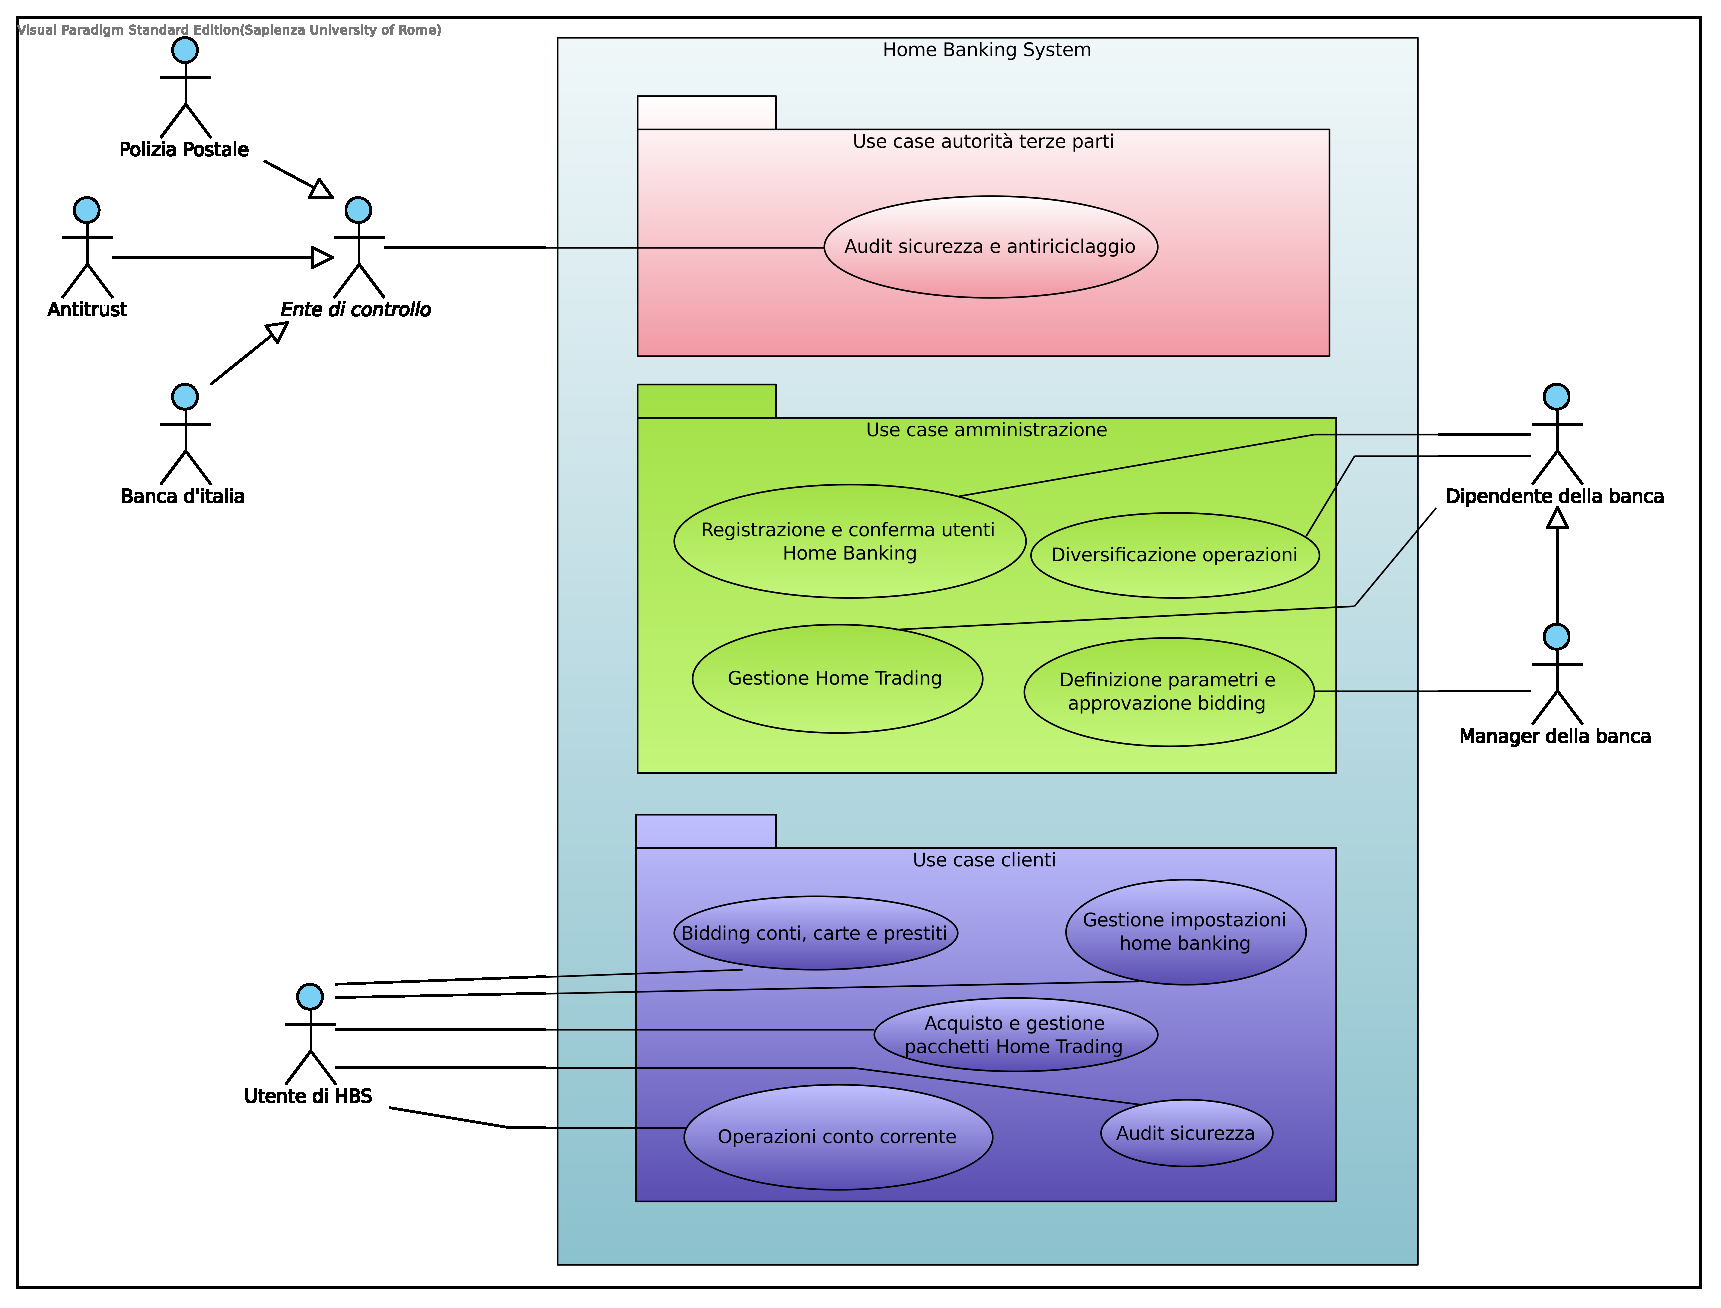
\includegraphics[width=\textwidth]{Images/Home_Banking_inception_use_cases.eps}
	\caption{Attori del sistema di Home Banking e relativi use cases.}
	\label{fig:use-cases}
\end{figure*}

\subsection{Use case di amministrazione}

Di seguito sono illustrati i diagrammi di use case relativi all'amministrazione della banca.

\begin{itemize}
	\item in figura~\ref{fig:use-cases:amministrazione} sono indicati gli use case più alto livello dell'amministrazione;

	\item in figura~\ref{fig:use-cases:amministrazione:gestione-utenti} sono indicati gli use case relativi alla gestione degli account utenti;

	\item in figura~\ref{fig:use-cases:amministrazione:gestione-bidding} sono indicati gli use case relativi alla creazione e alla gestione delle regole di bidding.
	Gli use case comprendono:
	\begin{itemize}
		\item use case \ref{}
	\end{itemize}

	\item in figura~\ref{fig:use-cases:amministrazione:gestione-operazioni-veloci} sono indicati gli use case relativi alla creazione e modifica delle operazioni veloci.
\end{itemize}

\begin{figure*}
	\centering
	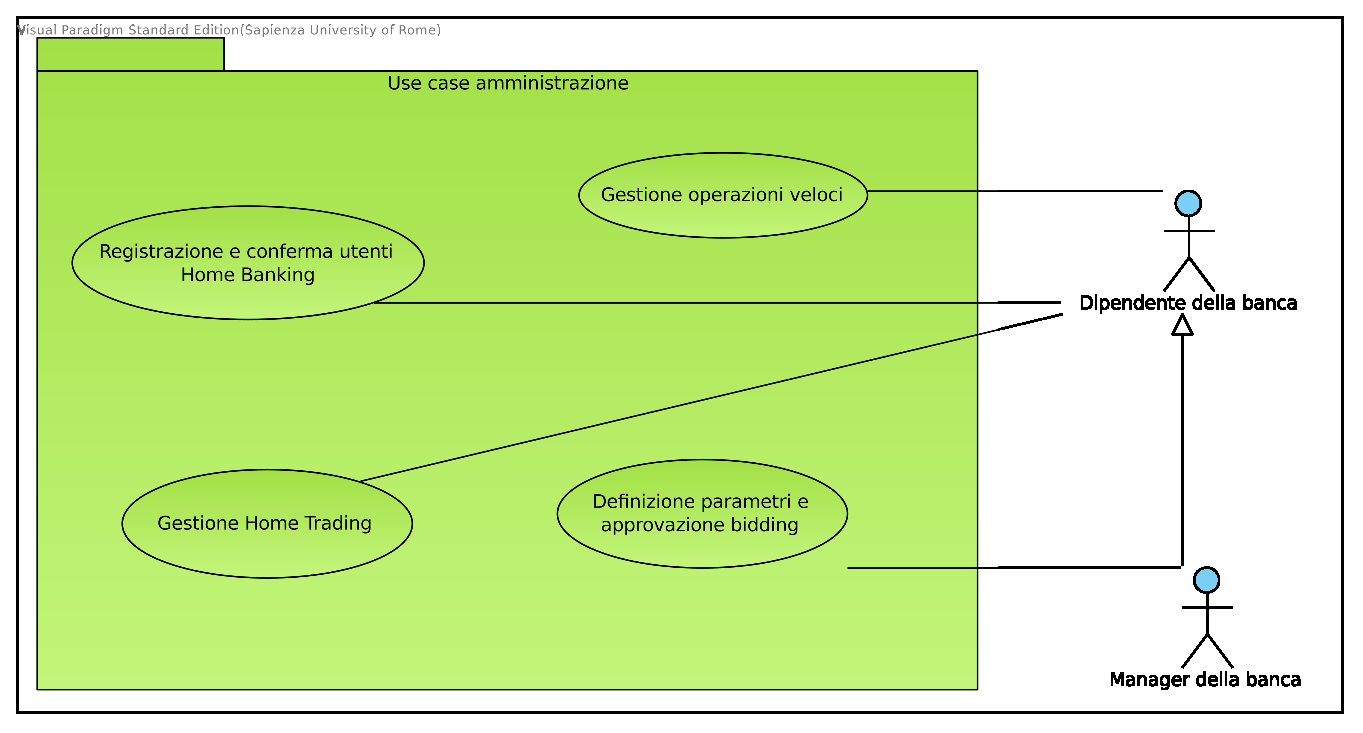
\includegraphics[width=\textwidth]{Images/use-cases/Amministrazione.eps}
	\caption{Diagramma degli use case di amministrazione.}
	\label{fig:use-cases:amministrazione}
\end{figure*}

\begin{figure*}
	\centering
	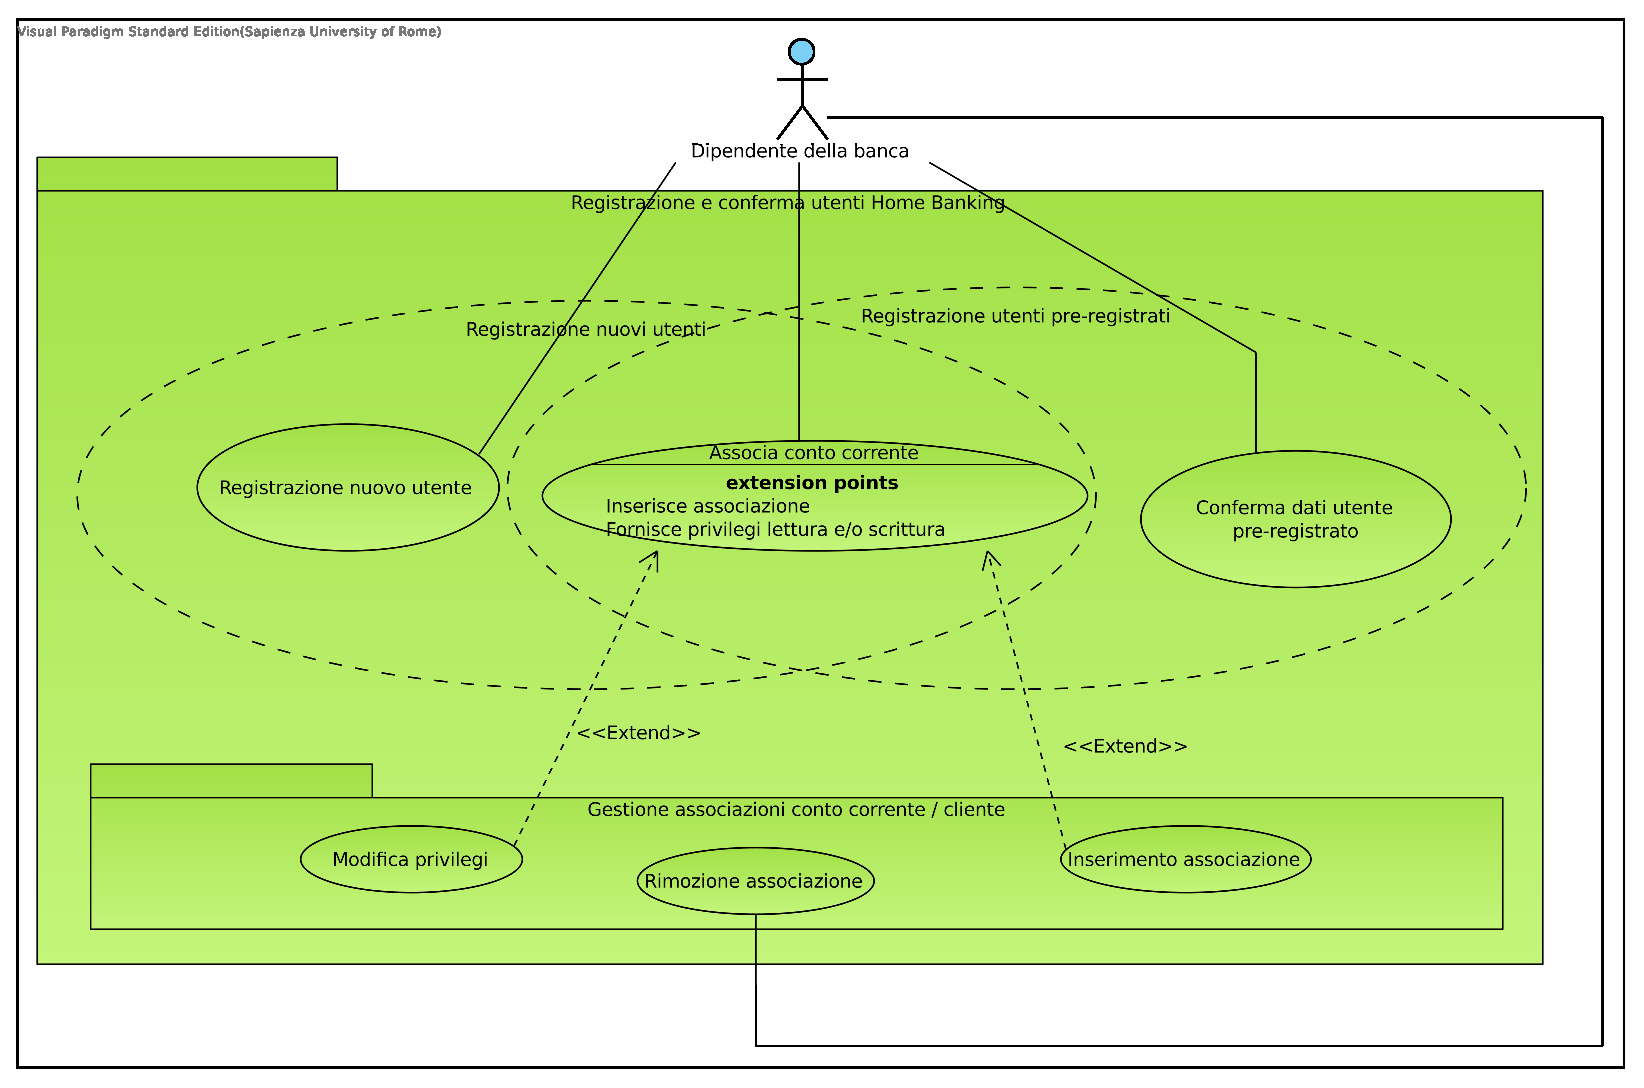
\includegraphics[width=\textwidth]{Images/use-cases/Registrazione_e_conferma_utenti_Home_Banking.eps}
	\caption{Diagramma degli use case per la registrazione e gestione degli utenti da parte dell'amministrazione della banca.}
	\label{fig:use-cases:amministrazione:gestione-utenti}
\end{figure*}

\begin{figure*}
	\centering
	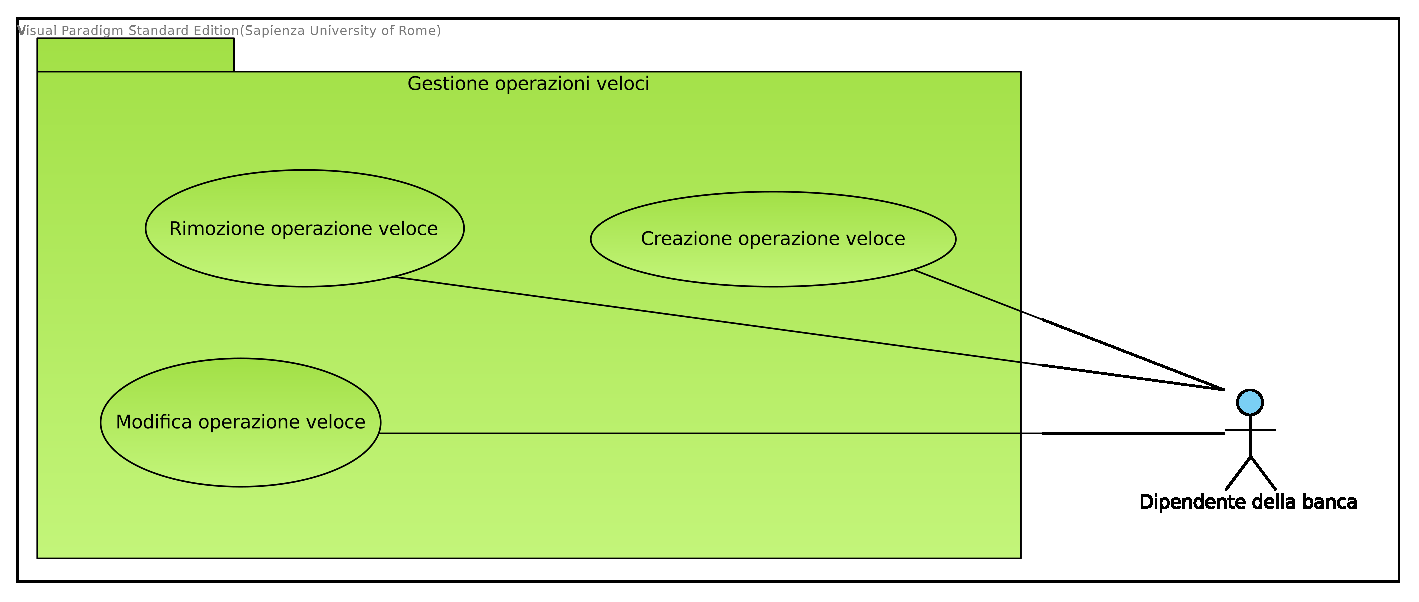
\includegraphics[width=\textwidth]{Images/use-cases/Gestione_operazioni_veloci.eps}
	\caption{Diagramma degli use case per la gestione delle operazioni veloci.}
	\label{fig:use-cases:amministrazione:gestione-operazioni-veloci}
\end{figure*}

\begin{figure*}
	\centering
	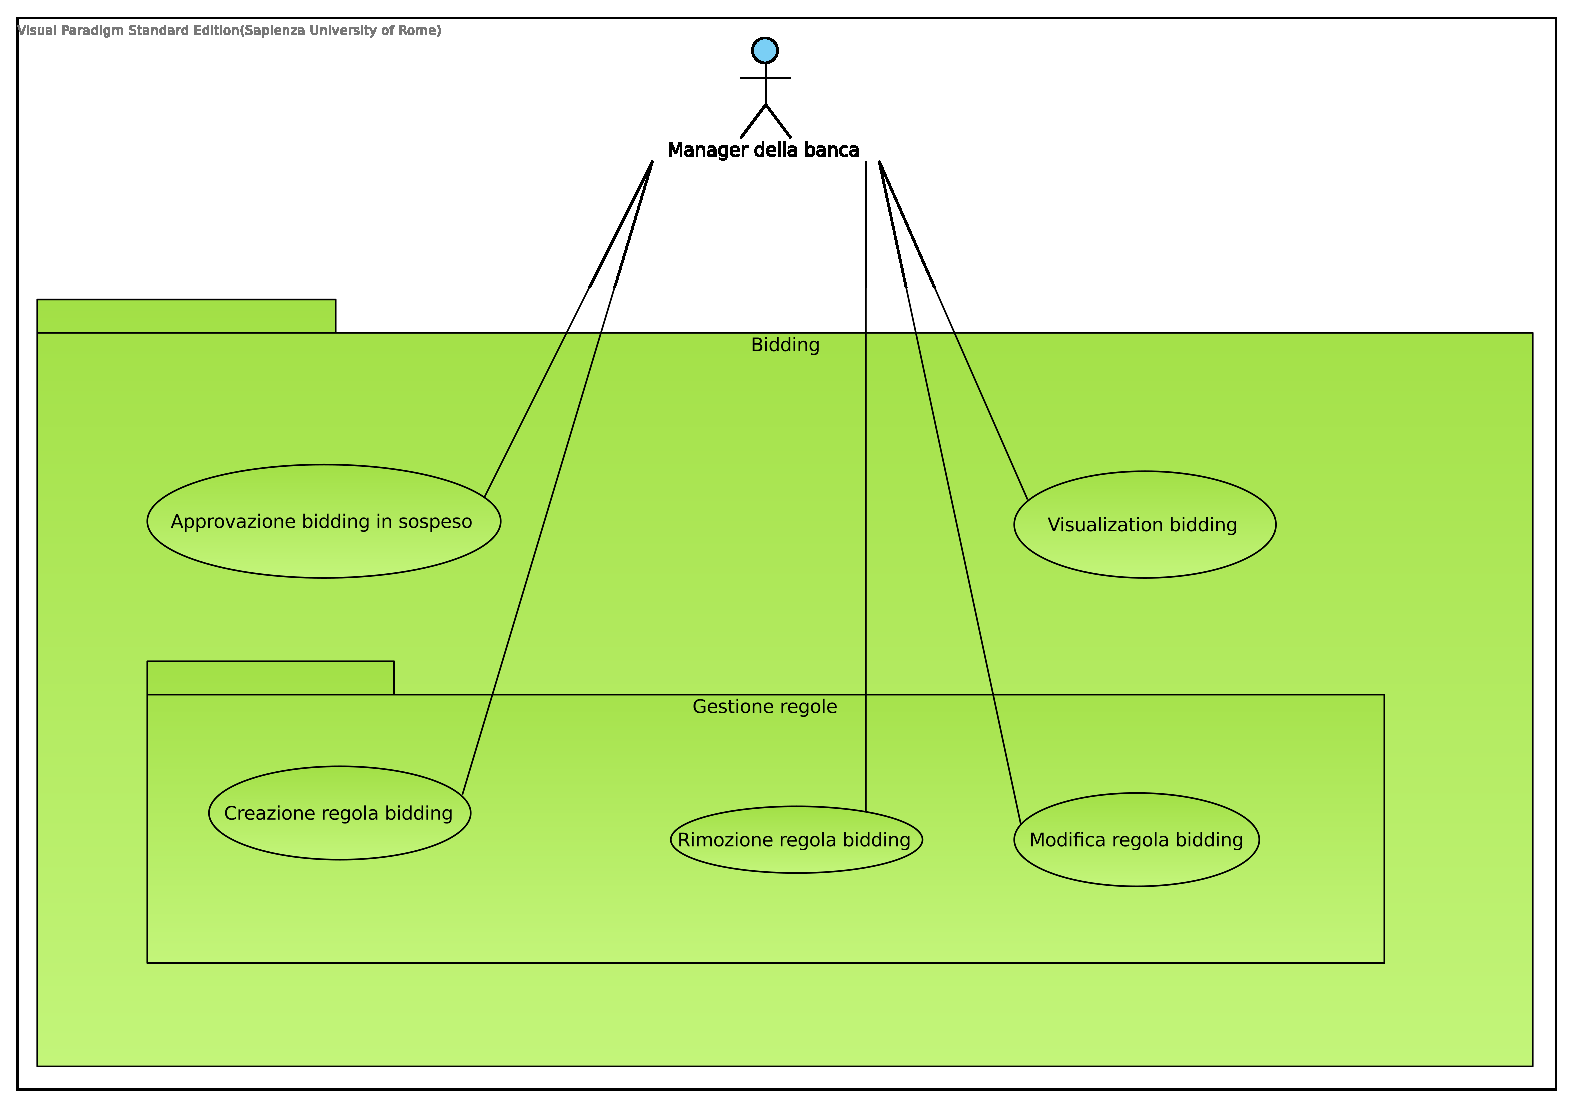
\includegraphics[width=\textwidth]{Images/use-cases/Definizione_parametri_e_approvazione_bidding.eps}
	\caption{Diagramma degli use case per la gestione delle regole di bidding.}
	\label{fig:use-cases:amministrazione:gestione-bidding}
\end{figure*}


\section{Specifica dei casi d'uso}

Di seguito \`e illustrata la specifica dei casi d'uso del sistema.

QUI CASI D'USO.

\subsection{Diagramma dei casi d'uso}

In figura INSERIRE RIFERIMENTO \`e illustrato il diagramma dei casi d'uso del progetto.



% \section{Corrispondenza casi d'uso / requisiti}

Nella matrice seguente \`e illustrata la corrispondenza fra casi d'uso e requisiti funzionali del sistema.
Un segno nella casella in riga $i$, colonna $j$, indica che il caso d'uso in riga $i$ realizza il requisito funzionale in colonna $j$.

Magia: posso riferirmi al requisito \ref{req:itm:utente:funzionali:iscrizione}.

\begin{tabular}{cc}
	Prova & ciao \\
\end{tabular}


\section{Registro modifiche}

\subsection{Elaboration}

\subsubsection{I iterazione}

Prima stesura documento.

\subsubsection{II iterazione}

Correzioni di errori.
Espanso use case model.

%----------------------------------------------------------------------------------------
%	REFERENCE LIST
%----------------------------------------------------------------------------------------

%\nocite{banca_italia}
\printcustombib{}

%----------------------------------------------------------------------------------------
%	FIGURES
%----------------------------------------------------------------------------------------

\end{document}
